\subsection{Designing effective step-by-step assembly instructions}
\begin{frame}\frametitle{\emph{Designing effective step-by-step assembly instructions} \cite{882352}} 


\begin{columns}[T]
\begin{column}{5cm}
\begin{itemize}
	\item O trabalho leva em considera��o aspectos psicol�gicos para propor modelos que produzem instru��es de montagem.
	\item Determina a ordem e a dire��o em que partes podem ser explodidades sem que restri��es sejam violadas.
	\item Apenas um n�vel de controle para expandir toda a vista explodida.
\end{itemize}
\vspace{3cm} 
\end{column}
\begin{column}{5cm}
\begin{overprint}
	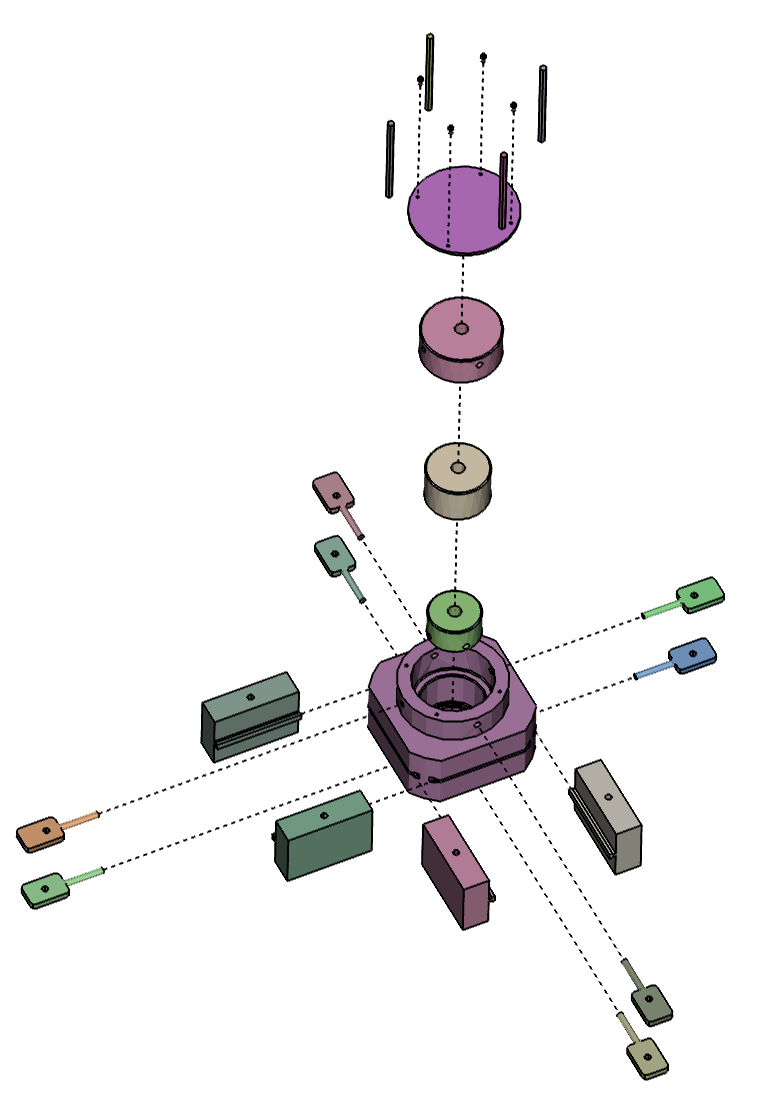
\includegraphics[height=150.0px]{img/assembly}
\end{overprint}
\end{column}
\end{columns}


\end{frame}